\documentclass[main.tex]{subfiles}
\ProvidesPackage{preamble}

\usepackage[nottoc]{tocbibind}
\usepackage[english]{babel}
\usepackage[utf8]{inputenc}
\usepackage[table]{xcolor}
\usepackage[nohead, nomarginpar, margin=1in, foot=.25in]{geometry}
\usepackage{tabularx}
\usepackage{graphicx}
\usepackage{float}
\usepackage[english]{babel}
\usepackage{paralist}
\usepackage{datetime}
\usepackage{afterpage}

\begin{document}

\section{Evaluation}

\subsection{Approach}
Evaluation of our product began after the team finished development and testing. As previously mentioned code was only merged after successfully passing automated tests and review by at least one other team member. We conclude that implemented features work correctly, and therefore implement their corresponding functional requirements correctly. Additional evaluation was required to assess whether or not identified non-functional requirements were fulfilled. This evaluation was performed on a requirement-by-requirement basis, and in some cases required the use of additional external tools (for example the installation of assistive technologies when evaluating accessibility requirements). In some cases, proper evaluation would have required access to resources not available to our team due to budget constraints. In these cases, the team attempted to perform evaluation as best possible and outline the difficulties experienced in this report. The team's main focus during evaluation was objectivity. To achieve this goal we relied on external tools and metrics for the evaluation of requirements where possible.

Although our evaluation process is extensive, we recognize that no amount of heuristic analysis is a perfect replacement for proper user testing, as these are two different approaches that address separate aspects of software usability and adequacy \cite{userTestingGood}. Additionally, some of the requirements outlined in the first semester, although important, are based on a user's subjective experience and are therefore impossible to evaluate without extensive user testing. Upon consulting with our guide and course coordinator, we were advised that user testing would be outside the scope of this course, and as such, the team decided not to conduct user testing at this stage. Extensive user testing will be performed during Thalia’s Alpha and Beta releases to fully evaluate our product's usability and user experience. While conducting user testing, there is a possibility the team identifies new user personas, and consequently new requirements. As we are following an Agile approach to software development, these features can easily be added to subsequent releases of Thalia by implementing a Release on Demand process \cite{releaseOnDemand}.
In the following sections, we will first discuss the results of the evaluation conducted for functional and non-functional requirements followed by a discussion of the overall success of the project.

\subsection{Functional Requirements}

As mentioned in last year's Technical Report, we introduced some milestones or releases for our product based on incremental sets of features. This was done to help us stay on track with development. The roadmap based on this schedule can be seen on \figurename{\ref{Roadmap}}.

\begin{figure}[H]
   \centering
   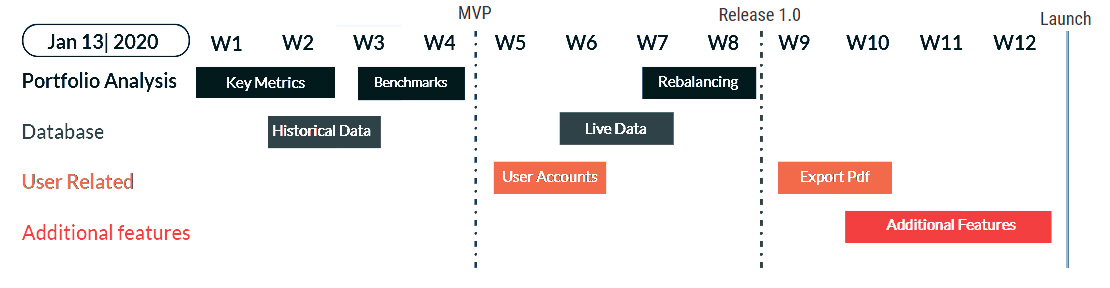
\includegraphics[width=\textwidth]{05Coding/05Pictures/initial_roadmap.jpg}
   \caption{Technical Report: Roadmap - revisited}
   \label{Roadmap}
\end{figure}

Due to our team's focus on process and code quality, the implementation of many features ended up taking longer than we initially predicted. Although the implementation of a single feature would generally be assigned as a single ticket, the writing of tests and refactoring of code to adjust for feedback would often mean tickets would take more than one week (our team's sprint length) to complete. Additionally, our team spent a lot of time implementing `under the hood` features to improve extensibility and maintainability. Most notably, the Anda module was designed as a separate library and Finda was designed to include advanced functionality seen in other ORMs (permission management and support for managing of several databases). Although these features contribute to the quality of our product, they ended up taking developer time away from the development of functional requirements in the early stages of our project.
Throughout our development process, the team would hold weekly retrospective meetings to try and better estimate velocity. These allowed us to react to this problem halfway through our allotted time. We came to the consensus decision to lock features that would be implemented and increase target weekly hours team members were expected to put into the project from 10 to 20. Additionally, we loosened some of the constraints necessary for deliverables to pass the review process and specialised the roles of team members to reduce the overhead of knowledge transfer. The result of this was that at the end of the project, all functional requirements except one were properly implemented.
The only functional requirement not yet implemented at the time of writing is the ability for a user to search for assets by category when creating a portfolio. Its omission is a result of a lack of resources, architectural limitations and our internal assessment of its importance. The team assessed each functional requirement not yet implemented and determined that listing assets by category is of low importance. This decision was based on the fact that it only provides users with a slight improvement to quality of life without giving any additional insight into the viability of their portfolios. Additionally, our team determined that implementation of this feature would require architectural changes the Thalia Web and Finda modules, meaning that its implementation would represent a bad cost to value ratio when compared with other remaining features. 
Even without this feature, we believe this prototype to be fully featured and usable and therefore ready for the next stages of development.

\subsection{Non-Functional Requirements}
The following are the results of our evaluation of non-functional requirements identified by our team listed by category, along with some general notes on our approach to evaluating each.

\subsubsection{Usability}
Usability requirements were particularly hard to assess. This was due to their subjective nature, relying on the experiences of users. Hence we will only conclusively be able to say that these requirements are fulfilled after performing user testing.

\begin{itemize}

\item The product must be easily usable for users who already have some financial investment experience.\\
\textit{Since Thalia’s design and features are based on feedback from finance students and enthusiasts interviewed in the first semester, we can infer that someone of similar experience would likely be familiar with most of Thalia's terminology, features and charts.}
\item The basic backtesting interface needs to look familiar to people already experienced with it. \\
\textit{The design of our interface closely follows that of our major competitor (Portfolio Visualizer), so it is safe to say that a user with moderate experience using it or other backtesting tools would have no trouble finding their way around.}

\item The product must have detailed instructions on how to use its advertised functions.\\
\textit{A link to an `About` section featuring instructions on how to use Thalia is featured in the taskbar on Thalia’s landing page. Additional material is also available in the user manual \ref{UserManual}.}
\item All major functions must be visible from the initial landing page.\\
\textit{All pages are accessible through the taskbar at the top of Thalia’s landing page.}
\item Must work in both desktop and mobile browsers.\\
\textit{Since Thalia’s dashboard is built using the Dash platform, it automatically scales to the size of the browser window, even when accessed from a mobile browser. All other pages have also been designed to work on mobile platforms.}
\item The results page should scale with mobile\\
\textit{Same as for the previous requirement.}

\end{itemize}

\subsubsection{Reliability}
\begin{itemize}

\item The product must have a greater than 99\% uptime.\\
\textit{Thalia is hosted by Amazon AWS, a reputable hosting provider who’s service level agreement (a legally binding contract) promises a monthly uptime of over 99.9\%\cite{amazonSLA}.}

\item All our assets need to have up-to-date daily data where the asset is still publicly tradeable.\\
\textit{All assets included in Thalia are gathered from APIs by the Data Harvester. All API usage constraints were thoroughly researched and tested to make sure we are able to access data daily and that the data provided was updated on all trading days. This practice will continue for any API that we wish to add to Thalia.}

\item All assets supported by the system must provide all publicly available historical data.\\
\textit{Both sources of data currently used by the Data Harvester (Yahoo Finance and Nomics) are publicly available and do not impose any restrictions on the use of said data.}

\end{itemize}

\subsubsection{Performance}
Performance and load times of Thalia's web page hosted on our cloud hosting provider were tested with the use of Google Lighthouse\cite{GoogleLighthouse}, a tool for evaluating web page quality.

\begin{itemize}
\item The website should load within 3 seconds on mobile.\\
\textit{Although Google Lighthouse estimated Thalia’s `time to interactive` (time needed for all interactive elements of the website to become accessible to the user) to be above the 3-second threshold, all other features of the page were loaded in this time. Additionally, Thalia scored well overall in performance.}


\begin{figure}[H]
   \centering
   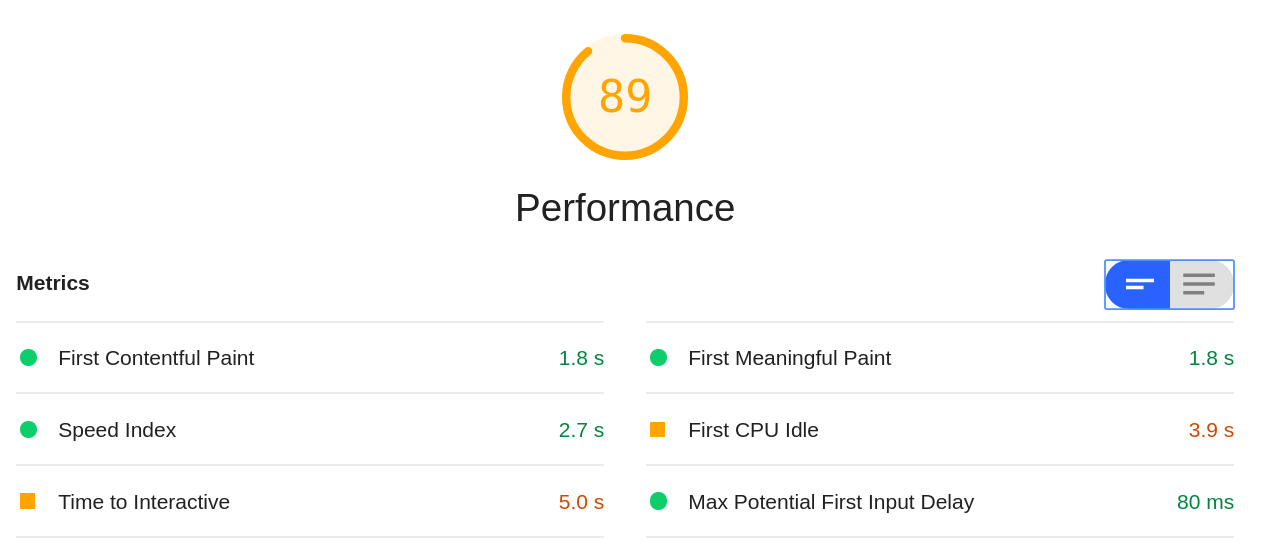
\includegraphics[scale=0.3]{07Evaluation/07Pictures/performanceLighthouse.png}
   \caption{Results of Lighthouse Performance Tests}
   \label{LighthousePerf}
\end{figure}



\item Large portfolios must be supported - up to 300 different assets.\\
\textit{There is no reasonable limit on the size of the portfolio supported, and our tool has been successfully tested on portfolios of over 300 assets. Although the tool does become unwieldy when entering portfolios of that scale since the table assets are entered into becomes too large to fit on a screen without scrolling. This problem is especially pronounced on mobile.}

\end{itemize}

\subsubsection{Supportability}

\begin{itemize}
\item The system should be well documented and easy to maintain.
\textit{The architecture and design of the system are documented in this report. Additional documentation on the individual modules is also available on the project wiki. Additionally, the team has created a maintenance manual\ref{MaintenanceManual} explaining in detail how to maintain and extend Thalia.}

\item The system should be fault-tolerant and be designed to support graceful degradation.
\textit{The system has been designed so that faults resulting from bad input and API problems do not crash the website. This means that users not directly affected can continue to run simulations.}

\item Installation and migration between hosting providers should be simple.
\textit{In an appropriate environment, both Thalia and its dependencies can be installed with a single command. Installation is extensively documented in the user manual\ref{UserManual}. Since CircleCI tests all working versions of Thalia in a Docker container, our application is easy to migrate to any platform that supports Docker.}

\item The system should be internationalized and be easy to extend to support new languages and currencies.
\textit{The current version of the Anda library supports currency conversion, as such adding new currencies is supported by our architecture. Versions of Thalia's website and dashboard in different languages can easily be implemented by hiring a translator. This is however outside the scope of our project witch is merely an high quality industrial prototype.}

\end{itemize}



\subsubsection{Implementation}
\begin{itemize}

\item The system needs to work on a cloud hosting provider.\\
\textit{The system is successfully deployed on Amazon AWS cloud hosting services.}

\end{itemize}

\subsubsection{Interfacing}
\begin{itemize}

\item The Data Gathering Module must never use APIs stated to-be-deprecated within a month.\\
\textit{Neither Yahoo Finance nor Nomics has made any statement to this effect. As such, we can assume both APIs will remain unchanged and available in the near future. In addition to this, Nomics API’s SLA (service level agreement) guarantees a high average uptime \cite{nomicsAPISpec}.}
\item The Data Gathering Module must not exceed its contractual usage limits.\\
\textit{Fulfilled as previously stated.}

\end{itemize}

\subsubsection{Operations}
\begin{itemize}

\item An administrator on-call will be necessary for unexpected issues.\\
\textit{This requirement would require the hiring of additional staff and is therefore outside the scope of this project. We have however included a form for submitting complaints on the Thalia website.}

\end{itemize}

\subsection{Packaging}
\begin{itemize}
\item The product needs to work inside a Linux container (e.g. Docker).\\
\textit{As previously mentioned, our CircleCI process’ tests are all run in a Docker container. This means that throughout development all working versions of Thalia have been tested and are therefore proved to be working inside one.}
\item All dependencies need to be installable with a single command.\\
\textit{Dependencies necessary for deployment are installed automatically when Thalia is installed with Pip. Testing and extra dependencies can be installed additionally, but are not necessary for running Thalia.}
\end{itemize}

\subsubsection{Legal}
Proper evaluation of the fulfilment of legal requirements would require consulting a legal professional, as none of the team have an in-depth understanding of British law. This is again outside the scope of this project. Nevertheless, the team has attempted to comply with the identified legal requirements to the best of our abilities so as to try and minimise potential future changes. The steps we have taken to fulfil these requirements are outlined below. 

\begin{itemize}

\item All user testing must be done with ethical approval from the University.\\
\textit{We were advised by the course coordinator that user testing is not necessary for this stage of our project. Additionally, we were advised that as long as no personal information is published, user testing could proceed without such approval. Therefore this is a false requirement.}

\item UI must display a clear legal disclaimer about the service not providing financial advice.\\
\textit{A disclaimer is clearly displayed on Thalia’s website. Since our tool doesn't propose a specific course of action to our users, it is likely it would constitute at most financial guidance and not financial advice\cite{FinAdvice}. In addition, our disclaimer is based on disclaimers found in the terms of service of competing software \cite{portfolioVisualizerToS} and should, therefore, require little modification after review by a legal professional.}

\item All third-party code should allow for commercial use without requiring source disclosure (e.g. no GPL-3).\\
\textit{With the use of the Pip package manager, we were able to confirm that the majority of third-party code does not require us to disclose our source code. The remaining package was identified to be nomics-python, which is used to access the Nomics API and is distributed under the MIT license, meaning it also allows commercial use without source code disclosure.}



\begin{figure}[H]
   \centering
   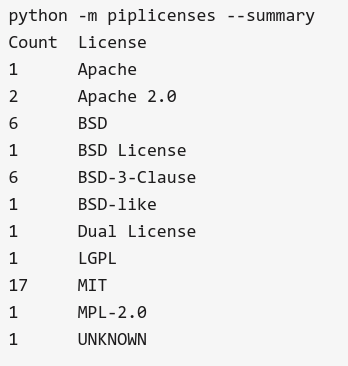
\includegraphics[scale=0.6]{07Evaluation/07Pictures/licensingPip.png}
   \caption{Licensing of 3rd party packages}
   \label{Licensing}
\end{figure}



\item User data handling should comply with GDPR.\\
\textit{The team has done its best to familiarize itself and comply with GDPR and related legislation\cite{guideToGDPR}.}
\item Provided services should not constitute financial advice under UK law to avoid being subject to financial advice legislation and potential liability.\\
\textit{Thalia is merely a tool for running simulations, and as such we at no point advises users on how to invest their real-life assets. This is also stated explicitly in our legal disclaimer.}

\end{itemize}


\subsubsection{Accessibility}
\begin{itemize}

\item Display items should be clearly labelled.\\
\textit{All UI elements are clearly labelled based on their purpose. All elements of the dashboard have been given descriptive names.}
\item UI should scale to accommodate different screen sizes and aspect ratios.\\
\textit{All pages on Thalia's website have been designed to scale to different-sized desktop and mobile displays. Dash apps automatically scale and rearrange elements to fit the display, meaning the main dashboard scales as well.}
\item UI elements and text superimposed over one another should have high contrast in their colours.\\
\textit{When selecting Thalia’s colour scheme, care was taken to allow for such contrast. On the dashboard, foreground elements and text are rendered in dark blue and black, while background elements are white or bone. A similar colour scheme is used for the other pages on Thalia’s website, with foreground and background colours inverted.}

\item UI should allow for the use of assistive technologies to accommodate for individuals with accessibility issues.\\
\textit{Selection of assistive technologies to test our website was made based on guidelines set out by the UK government identifying the 5 most commonly used assistive technologies \cite{govUKAccessability}. As these work by magnifying parts of the screen and reading out website text, they did not encounter any issues on our website. This means that Thalia in its current form reaches the high standard set for UK government institutions and associated businesses.}

\end{itemize}

\subsection{Evaluation Results}
The prototype of Thalia we have delivered along with this report fulfils the vast majority of identified functional requirements. We have also provided adequate reasoning for why we decided not to implement the remaining functional requirement. When possible, evaluation was also performed for each non-functional requirement. We believe that we have shown why these too are adequately fulfilled. In addition, our team has focused on the quality of our process throughout Thalia’s development, and as a result of this has been able to deliver high-quality code that has been extensively reviewed and tested. Based on these factors we evaluate that our project has been successful, and we have delivered a high quality, functioning piece of software that fits our identified business needs and market niche. 


\end{document}
